\documentclass[10pt, conference, compsocconf]{IEEEtran}
\usepackage{xcolor, soul}
\usepackage[utf8]{inputenc}
\usepackage{url}
\usepackage{graphicx}
\usepackage[caption=false,font=footnotesize]{subfig}
\usepackage{amsmath}
\usepackage{booktabs}
\usepackage{float}
\usepackage{cite}
\usepackage{csvsimple}
\usepackage{multirow}

\begin{document}

\title{Design and Calibration of a Digital Range Finder using ESP32}

\author{\IEEEauthorblockN{Atiqur Rahman (2202129), Sorder Rakib Hassan (2202140)}
\IEEEauthorblockA{Department of Electrical and Electronic Engineering\\
Chittagong University of Engineering \& Technology (CUET)}}

\maketitle

\begin{abstract}
This work presents the design and evaluation of a low-cost ESP32-based
ultrasonic digital range finder for non-contact distance measurement.
The system estimates distance using ultrasonic time-of-flight
measurement and was implemented with an ESP32, an ultrasonic sensor
arrangement, an I2C LCD, and firmware supporting calibration and data
collection. Performance was studied in both pulse-echo and pitch-catch
modes, with moving-average processing applied to improve measurement
stability.

Calibration was carried out using known reference distances so that the
firmware could compensate for systematic error associated with sensor
characteristics, alignment, timing offsets, and environmental effects.
Experimental results show that the prototype achieved useful
measurements up to 165~cm, with the most stable performance in the
medium and far ranges. After outlier removal, the best overall mean
absolute error was 0.465~cm, while practical clearance constraints
indicate an effective usable range of about 90~cm in obstructed
environments. The developed system therefore provides a simple and
reliable solution for low-cost distance sensing applications.
\end{abstract}

\section{Introduction}
Accurate distance measurement is central to many electrical and electronic engineering applications, ranging from robotics and industrial automation to fluid-level control and non-contact gauging. Ultrasonic rangefinders provide a low-cost, robust method to make such measurements because they are insensitive to ambient light and electromagnetic interference \cite{mi13040520}. These sensors operate by emitting a short burst of high-frequency sound and measuring the time elapsed until an echo returns from a target. Non-contact distance measurement avoids mechanical wear and is safer for applications involving moving parts or hazardous environments.

The ESP32 microcontroller family integrates a dual-core 32-bit processor, Wi-Fi, Bluetooth and a rich set of peripherals including UART, SPI, I\textsuperscript{2}C and ADC interfaces. These modules operate from 3.0--3.6 V, have up to 26 GPIO pins and can clock at up to 240 MHz. Their high computing power and low power consumption make them suitable as the control unit for a digital range finder. An I\textsuperscript{2}C LCD provides a simple user interface to display the measured distance \cite{esp32_datasheet}.

This project aims to design and build a digital range finder that uses ultrasonic time-of-flight measurement with the ESP32 and to calibrate the device over a 10--100 cm range. The report describes the physics of ultrasonic ranging, factors affecting measurement accuracy and advanced signal-processing techniques, then outlines an action plan for implementing and calibrating the instrument.

\section{Measurement Principle and Mode}

Ultrasonic ranging can be implemented using several methods,
including pulse-echo time-of-flight (ToF), phase-shift-based
measurement, and frequency-modulated/chirp-based ranging
approaches \cite{mi13040520}. Each method has different
trade-offs in hardware complexity, processing requirements,
and noise robustness.

In this project, we employed the ToF method because of its
simple implementation with the ESP32 platform. The system
was configured in a pitch-catch mode, where separate
transmitting and receiving transducers are used.

\subsection{Time-of-Flight Principle}

For a generic pulse-echo ToF configuration, distance is
computed from travel time as

\begin{equation}
d = \frac{c\,t}{2}
\end{equation}

where $c$ is the speed of sound in air and $t$ is the measured
round-trip time.

For the pitch-catch geometry used in this work,
Fig.~\ref{fig:pitch_catch_mode} shows two separated
transducers with spacing $h$. If the total ToF is $t$, then each
acoustic path has length

\begin{equation}
s = \frac{c\,t}{2}
\end{equation}

Using the right-triangle relation in the figure, the forward
standoff distance to the target is

\begin{equation}
d = \sqrt{s^2 - \left(\frac{h}{2}\right)^2}
= \sqrt{\left(\frac{c\,t}{2}\right)^2 - \left(\frac{h}{2}\right)^2}
\end{equation}

When $h \ll 2d$, this reduces approximately to
$d \approx \frac{c\,t}{2}$.

\begin{figure}[!t]
\centering
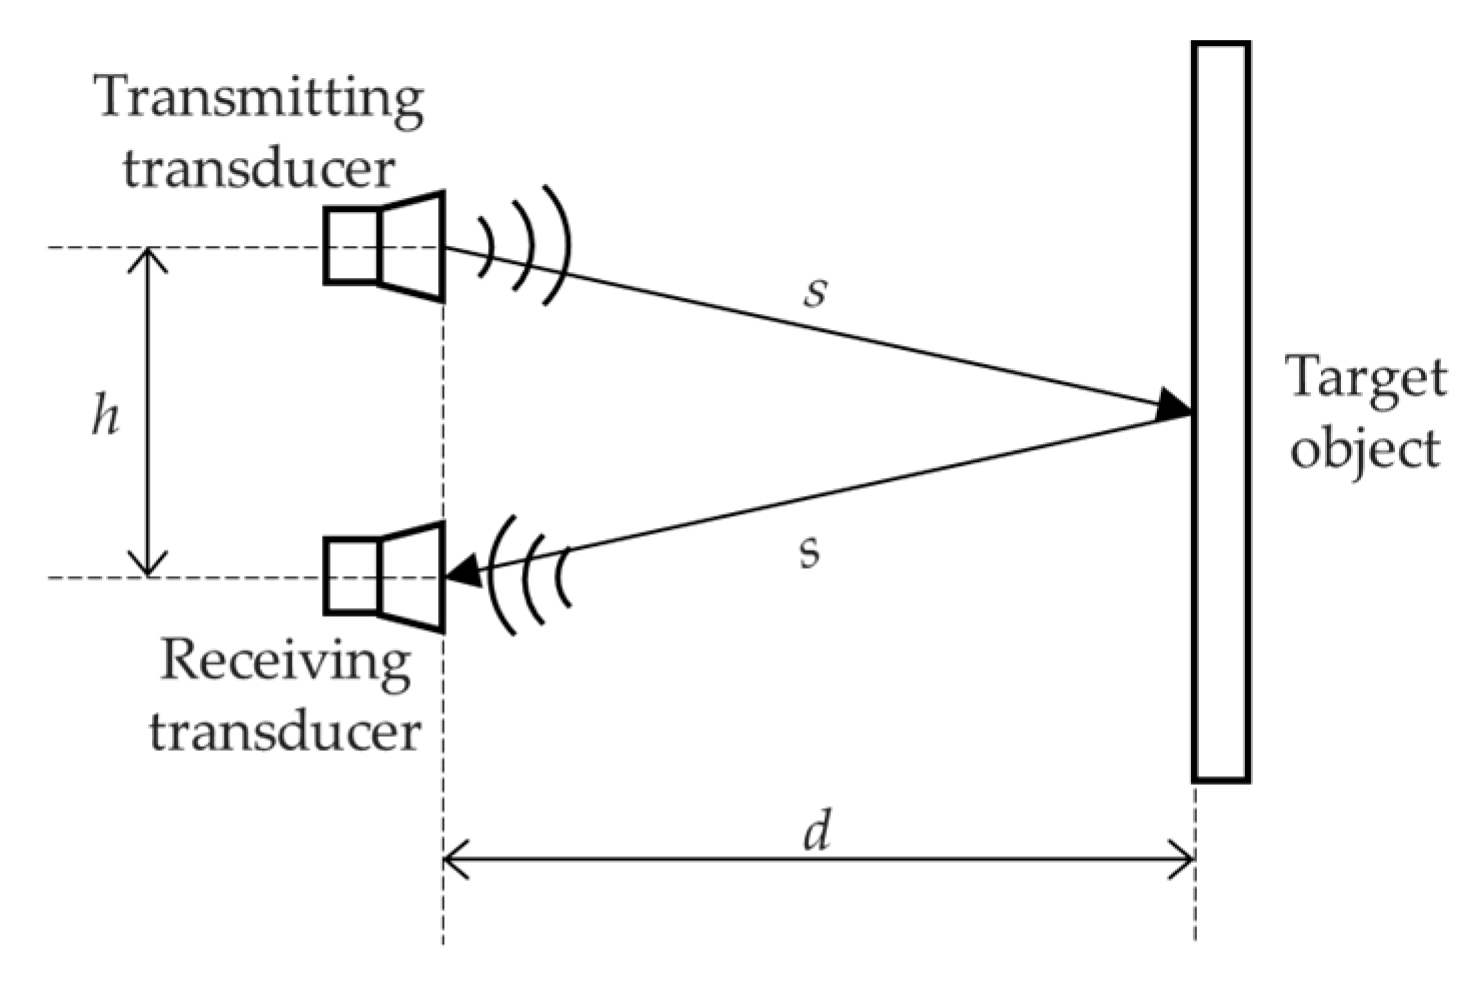
\includegraphics[width=0.95\linewidth]{figures/schematic_diagram_for_pair_of_transducer.png}
\caption{Pitch-catch ultrasonic ranging geometry (adapted from \cite{mi13040520}).}
\label{fig:pitch_catch_mode}
\end{figure}

\subsection{Speed of Sound in Air}

The speed of sound in air depends primarily on the ambient
temperature. In dry air at $0^\circ$C, the speed of sound is
approximately

\begin{equation}
c \approx 331.45 \; \mathrm{m\,s^{-1}}
\end{equation}

A commonly used linear approximation relating sound speed
to air temperature is \cite{mi13040520}

\begin{equation}
c \approx 331.45 + 0.607\,T_C
\end{equation}

where $T_C$ is the air temperature in degrees Celsius. This
relation indicates that the speed of sound increases by about
$0.6\,\mathrm{m\,s^{-1}}$ for every $1^\circ$C increase in
temperature.

Environmental factors such as humidity and atmospheric
pressure also affect the propagation speed of sound, though
their influence is comparatively smaller. Across typical
ranges of $0$--$100\%$ relative humidity and
$50$--$110$\,kPa pressure, the variation in sound speed is
generally less than $0.7\%$ \cite{mi13040520}.

In the implemented system, these environmental effects were
handled through calibration rather than direct temperature or
humidity measurement. Their impact could be reduced further in
future versions by adding dedicated environmental sensors and
updating the value of $c$ accordingly.

\section{Methodology and Design}
\subsection{Hardware Implementation}

The prototype consists of the following main components:

\begin{itemize}
\item ESP32 development board
\item HC-SR04 ultrasonic sensor
\item Low-power laser module mounted at the centerline of the ultrasonic transducers
\item I\textsuperscript{2}C 16$\times$2 LCD module with backpack
\item Breadboard, jumper wires, and regulated power supply
\end{itemize}

\subsubsection{Circuit Connections}

The ESP32 development board is powered using a regulated 3.3\,V supply.
The ultrasonic sensor module is powered from the ESP32 supply rail, and
its ground is connected to the ESP32 ground to establish a common reference.

The Trigger pin of the ultrasonic sensor is connected to a digital GPIO pin
configured as an output. The Echo pin is connected to a GPIO pin
configured as an input.

The I\textsuperscript{2}C LCD module is connected to the ESP32
I\textsuperscript{2}C interface. The SDA and SCL lines are connected
to GPIO 21 and GPIO 22 respectively.

The laser module is mechanically fixed so that its beam emerges from the
middle of the two ultrasonic transducers. This laser is used only as a
visual pointer to align the measurement axis with the target point.

\begin{figure}[!t]
\centering
\includegraphics[width=0.95\linewidth]{figures/wowki_simulation_circuit_diagram.png}
\caption{Wokwi simulation circuit diagram used to verify the ESP32-based measurement system \cite{wokwi_simulation}.}
\label{fig:wokwi_simulation}
\end{figure}

\subsubsection{Prototype Assembly}

All components are assembled on a breadboard during the prototyping stage.
The ultrasonic transducer is positioned so that it has a clear line of sight
to the target surface. The laser pointer is adjusted during assembly so its
spot coincides with the center of the ultrasonic sensing direction.
Care is taken to minimize nearby reflective objects that could introduce
unwanted echoes. If necessary, simple shielding or damping materials can be
placed around the sensor to reduce acoustic reflections from surrounding
surfaces.

\begin{figure}[!t]
\centering
\subfloat[Top view of the assembled circuit.]{
\includegraphics[width=0.47\linewidth]{figures/actual_circuit_top.jpeg}
\label{fig:actual_circuit_top}
}
\hfill
\subfloat[Side view of the assembled circuit.]{
\includegraphics[width=0.47\linewidth]{figures/actual_circuit_side.jpeg}
\label{fig:actual_circuit_side}
}
\caption{Photographs of the actual hardware prototype used in the experiment.}
\label{fig:actual_circuit_photos}
\end{figure}

\subsection{Software Flow}
The ESP32 generates a trigger pulse sequence for each measurement cycle.
First, the trigger pin is set LOW for $2\,\mu$s, then set HIGH for
$10\,\mu$s, and then returned LOW. The echo pulse width is measured using the
Arduino \texttt{pulseIn()} function on the echo pin with a timeout of
$30{,}000\,\mu$s. The detailed software and firmware implementation used
in this project is available in the project repository
\cite{eee354_github_repo}.

\begin{figure}[!t]
\centering
\includegraphics[width=0.95\linewidth]{figures/firmware_mode_flow.jpeg}
\caption{Firmware flow diagram showing the operating sequence and mode selection of the ESP32-based system.}
\label{fig:firmware_mode_flow}
\end{figure}

If no valid echo pulse is received within the timeout, that cycle is ignored.
If a valid pulse is received, the time value is stored and the distance is
computed using Eq.~(3). The resulting distance is then sent to the active user
interface mode.

\begin{figure}[!t]
\centering
\includegraphics[width=0.9\linewidth]{figures/sensor_reading_cycle_flow.jpeg}
\caption{Sensor reading cycle diagram for one ultrasonic measurement cycle.}
\label{fig:sensor_reading_cycle}
\end{figure}

Two software operating modes are implemented:
\begin{itemize}
\item \textbf{LCD mode (local mode):} after powering the ESP32, pressing the
BOOT button once starts local display mode, where distance is shown on the
LCD.
\item \textbf{Website mode (Wi-Fi mode):} after reset, pressing the BOOT
button twice starts web mode. The ESP32 starts the web interface and displays
its IP address. A user connects over Wi-Fi, opens the IP address in a browser,
and can view live readings, record readings, and perform calibration tasks
\cite{eee354_github_repo}.
\end{itemize}

\section{Calibration and Results}
\subsection{Calibration Procedure}
The developed firmware includes a web-based calibration interface for
updating the ranging parameters of the ESP32-based measurement system
\cite{eee354_github_repo}.
After powering the device, the ESP32 can be placed into Wi-Fi mode by
pressing the boot button twice. In this mode, the user connects to the
firmware-hosted local network interface and accesses the calibration page
through a web browser.

For calibration, the sensor is positioned at a known distance from a
target object, measured beforehand using a reference scale. The same
reference distance is then entered into the firmware interface, and the
calibration command is executed. During this process, the transmitter
emits an ultrasonic pulse and the system measures the corresponding
time-of-flight from the received signal. Using the known reference
distance and the measured travel time, the firmware estimates an
effective sound velocity for the current operating condition.

This procedure is important because practical measurement error may
arise from sensor characteristics, alignment imperfections,
hardware-related timing offsets, and environmental variation.
Temperature and humidity effects were handled indirectly through
calibration in this work. These effects could be reduced further by
using additional environmental sensors in a future version of the
system. By calibrating the device at a known distance, these systematic
effects can be partially compensated, allowing the firmware to adjust
its distance calculation for improved accuracy.

\subsection{Data and Analysis}
The sensor readings were processed in both pulse-echo mode and
pitch-catch mode in order to evaluate and compare their performance.

\begin{table}[!t]
\centering
\caption{Readings \& corresponding errors when data is processed in pulse-echo mode}
\scriptsize
\setlength{\tabcolsep}{3pt}
\begin{tabular}{|c|c|c|c|c|}
\hline
\shortstack{\textbf{Actual}\\\textbf{(cm)}} & \shortstack{\textbf{Raw}\\\textbf{reading}\\\textbf{(cm)}} & \shortstack{\textbf{Raw reading with}\\\textbf{moving avg}\\\textbf{(cm)}} & \shortstack{\textbf{Raw}\\\textbf{error}\\\textbf{(\%)}} & \shortstack{\textbf{Moving avg}\\\textbf{error}\\\textbf{(\%)}} \\ \hline
1.5 & 1.71 & 1.71 & 14.00 & 14.00 \\ \hline
2 & 1.71 & 1.71 & 14.50 & 14.50 \\ \hline
3 & 1.71 & 2.76 & 43.00 & 8.00 \\ \hline
4 & 3.99 & 3.99 & 0.25 & 0.25 \\ \hline
5 & 4.96 & 5.56 & 0.80 & 11.20 \\ \hline
6 & 4.65 & 4.65 & 22.50 & 22.50 \\ \hline
7 & 7.92 & 7.72 & 13.14 & 10.29 \\ \hline
8 & 7.92 & 7.91 & 1.00 & 1.12 \\ \hline
9 & 8.92 & 8.92 & 0.89 & 0.89 \\ \hline
10 & 9.96 & 9.95 & 0.40 & 0.50 \\ \hline
15 & 15.44 & 15.46 & 2.93 & 3.07 \\ \hline
20 & 19.47 & 19.47 & 2.65 & 2.65 \\ \hline
25 & 24.59 & 24.6 & 1.64 & 1.60 \\ \hline
30 & 29.68 & 29.69 & 1.07 & 1.03 \\ \hline
35 & 34.29 & 34.61 & 2.03 & 1.11 \\ \hline
40 & 40.07 & 40.06 & 0.18 & 0.15 \\ \hline
45 & 44.52 & 44.53 & 1.07 & 1.04 \\ \hline
50 & 50.53 & 50.2 & 1.06 & 0.40 \\ \hline
55 & 54.86 & 54.54 & 0.25 & 0.84 \\ \hline
60 & 59.77 & 59.68 & 0.38 & 0.53 \\ \hline
70 & 69.51 & 53.31 & 0.70 & 23.84 \\ \hline
80 & 79.13 & 79.12 & 1.09 & 1.10 \\ \hline
90 & 89.38 & 87.18 & 0.69 & 3.13 \\ \hline
100 & 99.45 & 99.47 & 0.55 & 0.53 \\ \hline
120 & 120.48 & 120.47 & 0.40 & 0.39 \\ \hline
140 & 140.21 & 140.24 & 0.15 & 0.17 \\ \hline
148 & 148.99 & 149.27 & 0.67 & 0.86 \\ \hline
165 & 166.01 & 166.5 & 0.61 & 0.91 \\ \hline
\end{tabular}
\end{table}

\begin{table}[!t]
\centering
\caption{Readings \& corresponding errors when data is processed in pitch-catch mode}
\scriptsize
\setlength{\tabcolsep}{3pt}
\begin{tabular}{|c|c|c|c|c|}
\hline
\shortstack{\textbf{Actual}\\\textbf{(cm)}} & \shortstack{\textbf{Pitch-}\\\textbf{catch}\\\textbf{(cm)}} & \shortstack{\textbf{Pitch-catch with}\\\textbf{moving avg}\\\textbf{(cm)}} & \shortstack{\textbf{Pitch-catch}\\\textbf{error}\\\textbf{(\%)}} & \shortstack{\textbf{Pitch-catch moving avg}\\\textbf{error}\\\textbf{(\%)}} \\ \hline
1.5 & 1.39 & 1.39 & 7.33 & 7.33 \\ \hline
2 & 1.39 & 1.39 & 30.50 & 30.50 \\ \hline
3 & 1.39 & 2.56 & 53.67 & 14.67 \\ \hline
4 & 3.87 & 3.87 & 3.25 & 3.25 \\ \hline
5 & 4.86 & 5.47 & 2.80 & 9.40 \\ \hline
6 & 4.54 & 4.54 & 24.33 & 24.33 \\ \hline
7 & 7.85 & 7.65 & 12.14 & 9.29 \\ \hline
8 & 7.85 & 7.85 & 1.88 & 1.88 \\ \hline
9 & 8.87 & 8.87 & 1.44 & 1.44 \\ \hline
10 & 9.91 & 9.9 & 0.90 & 1.00 \\ \hline
15 & 15.41 & 15.42 & 2.73 & 2.80 \\ \hline
20 & 19.44 & 19.44 & 2.80 & 2.80 \\ \hline
25 & 24.57 & 24.58 & 1.72 & 1.68 \\ \hline
30 & 29.67 & 29.67 & 1.10 & 1.10 \\ \hline
35 & 34.28 & 34.6 & 2.06 & 1.14 \\ \hline
40 & 40.06 & 40.05 & 0.15 & 0.12 \\ \hline
45 & 44.51 & 44.52 & 1.09 & 1.07 \\ \hline
50 & 50.52 & 50.19 & 1.04 & 0.38 \\ \hline
55 & 54.85 & 54.53 & 0.27 & 0.85 \\ \hline
60 & 59.76 & 59.67 & 0.40 & 0.55 \\ \hline
70 & 69.5 & 53.3 & 0.71 & 23.86 \\ \hline
80 & 79.13 & 79.11 & 1.09 & 1.11 \\ \hline
90 & 89.38 & 87.18 & 0.69 & 3.13 \\ \hline
100 & 99.45 & 99.46 & 0.55 & 0.54 \\ \hline
120 & 120.47 & 120.47 & 0.39 & 0.39 \\ \hline
140 & 140.21 & 140.24 & 0.15 & 0.17 \\ \hline
148 & 148.99 & 149.27 & 0.67 & 0.86 \\ \hline
165 & 166 & 166.5 & 0.61 & 0.91 \\ \hline
\end{tabular}
\end{table}

\begin{table}[!t]
\centering
\caption{Required clearance at different measurement intervals.}
\scriptsize
\setlength{\tabcolsep}{4pt}
\begin{tabular}{|c|c|}
\hline
\shortstack{\textbf{Distance range}\\\textbf{(cm)}} & \shortstack{\textbf{Required clearance}\\\textbf{(cm)}} \\ \hline
0--30 & 7 \\ \hline
30--60 & 26 \\ \hline
60--90 & 36 \\ \hline
90--120 & 45 \\ \hline
120--150 & 65 \\ \hline
\end{tabular}
\end{table}

\begin{table}[!t]
\centering
\caption{Mean absolute error different distance ranges and processing methods.}
\scriptsize
\setlength{\tabcolsep}{4pt}
\begin{tabular}{|c|c|c|c|}
\hline
\shortstack{\textbf{Range}\\\textbf{(cm)}} & \textbf{Method} & \shortstack{\textbf{MAE}\\\textbf{before}} & \shortstack{\textbf{MAE after}\\\textbf{outlier removal}} \\ \hline
\multirow{4}{*}{All (0--200)} & \shortstack{Raw reading\\(pulse echo)\\with moving avg} & 1.128571 & 0.465000 \\ \cline{2-4}
& \shortstack{Raw reading\\(pulse echo)} & 0.478214 & 0.478214 \\ \cline{2-4}
& \shortstack{Pitch-catch\\with moving avg} & 1.154643 & 0.492692 \\ \cline{2-4}
& \shortstack{Pitch-catch} & 0.514286 & 0.514286 \\ \hline
\multirow{4}{*}{Close (0--10)} & \shortstack{Raw reading\\(pulse echo)\\with moving avg} & 0.360000 & 0.360000 \\ \cline{2-4}
& \shortstack{Pitch-catch\\with moving avg} & 0.425000 & 0.425000 \\ \cline{2-4}
& \shortstack{Raw reading\\(pulse echo)} & 0.431000 & 0.431000 \\ \cline{2-4}
& \shortstack{Pitch-catch} & 0.528000 & 0.528000 \\ \hline
\multirow{4}{*}{Far (60--200)} & \shortstack{Raw reading\\(pulse echo)} & 0.605556 & 0.605556 \\ \cline{2-4}
& \shortstack{Pitch-catch} & 0.605556 & 0.605556 \\ \cline{2-4}
& \shortstack{Raw reading\\(pulse echo)\\with moving avg} & 2.746667 & 1.003750 \\ \cline{2-4}
& \shortstack{Pitch-catch\\with moving avg} & 2.751111 & 1.007500 \\ \hline
\multirow{4}{*}{Medium (10--60)} & \shortstack{Raw reading\\(pulse echo)\\with moving avg} & 0.331818 & 0.331818 \\ \cline{2-4}
& \shortstack{Pitch-catch\\with moving avg} & 0.340909 & 0.340909 \\ \cline{2-4}
& \shortstack{Raw reading\\(pulse echo)} & 0.354545 & 0.354545 \\ \cline{2-4}
& \shortstack{Pitch-catch} & 0.363636 & 0.363636 \\ \hline
\end{tabular}
\end{table}

In addition to the distance calibration results, the required clearance
along the acoustic path was also investigated. This was done to ensure
that the sensor measured the intended target distance rather than
detecting unwanted objects located near the propagation path or within
the peripheral region outside the direct line of measurement.

\subsection{Performance Graph}
The following plots summarize the measured sensor response, the
error trend across distance, the average error in different operating
ranges, and the clearance requirement.

Figure~\ref{fig:sensor_reading_plots} shows that, over most of the
measured range, the processed sensor outputs follow the ideal
distance-response line closely. The agreement is strongest in the
medium and far ranges, where the plotted points remain near the
reference line for all four processing cases. Larger deviations are
mainly observed in the close range, especially below approximately
10~cm, where the measured points are more scattered and the relative
error becomes significantly higher. This behavior is also consistent
with the tabulated results, where the shortest-distance measurements
produce the largest percentage errors.

The error curves in Figure~\ref{fig:error_plots} indicate that the main
performance limitation is concentrated at short distances and at a few
isolated outlier points. In the full-range plot, most data beyond the
close region remain within a low error band, generally around
1--3\%, whereas very large peaks appear at the smallest measured
distances and at one anomalous point in the far range when moving
average processing is applied. The medium-range plot shows the most
stable overall response, with comparatively smooth behavior and small
deviations for all methods. In contrast, the far-range plot suggests
that the raw pulse-echo and raw pitch-catch results remain relatively
stable, while the moving-average cases are more sensitive to occasional
abnormal measurements.

The mean absolute error comparison in
Figure~\ref{fig:mae_ranges} and Table~IV further clarifies this trend.
After outlier removal, the best overall performance across the full
range is obtained using raw pulse-echo readings with moving average,
which gives an MAE of 0.465~cm. In the close range, the same method
also produces the smallest MAE of 0.360~cm, while in the medium range
it again provides the lowest value of 0.3318~cm. However, in the far
range, the unfiltered raw pulse-echo and raw pitch-catch methods both
perform better, each yielding an MAE of 0.6056~cm, whereas the
moving-average methods rise to approximately 1.0~cm after outlier
removal. This indicates that averaging is beneficial in short and
medium distances, but it may amplify the effect of occasional abnormal
samples in long-range measurements. From a practical perspective, the
full-range average error of approximately 0.45--0.50~cm suggests that
the system is more suitable for applications that can tolerate about
$\pm 0.45$~cm uncertainty than for precision-critical measurement
tasks.

Figure~\ref{fig:clearance_calculation} complements the distance results
by illustrating the required clearance around the measurement axis. The
clearance increases with distance, from 7~cm in the 0--30~cm interval
to 65~cm in the 120--150~cm interval. This trend is expected because
the ultrasonic beam spreads as distance increases, enlarging the region
from which reflections may be received. Consequently, accurate
long-range measurement requires a wider unobstructed path to avoid
detecting nearby peripheral objects instead of the intended target. The
clearance plot also indicates that the theoretical measurement angle of
approximately $15^\circ$ reported in the HC-SR04 datasheet
\cite{HC-SR04_datasheet} agrees reasonably well only up to about
30~cm. Beyond this region, the experimentally observed boundary rises to
about $22^\circ$, indicating a wider effective beam in practice than in
the simplified theoretical model.

\begin{figure}[!t]
\centering
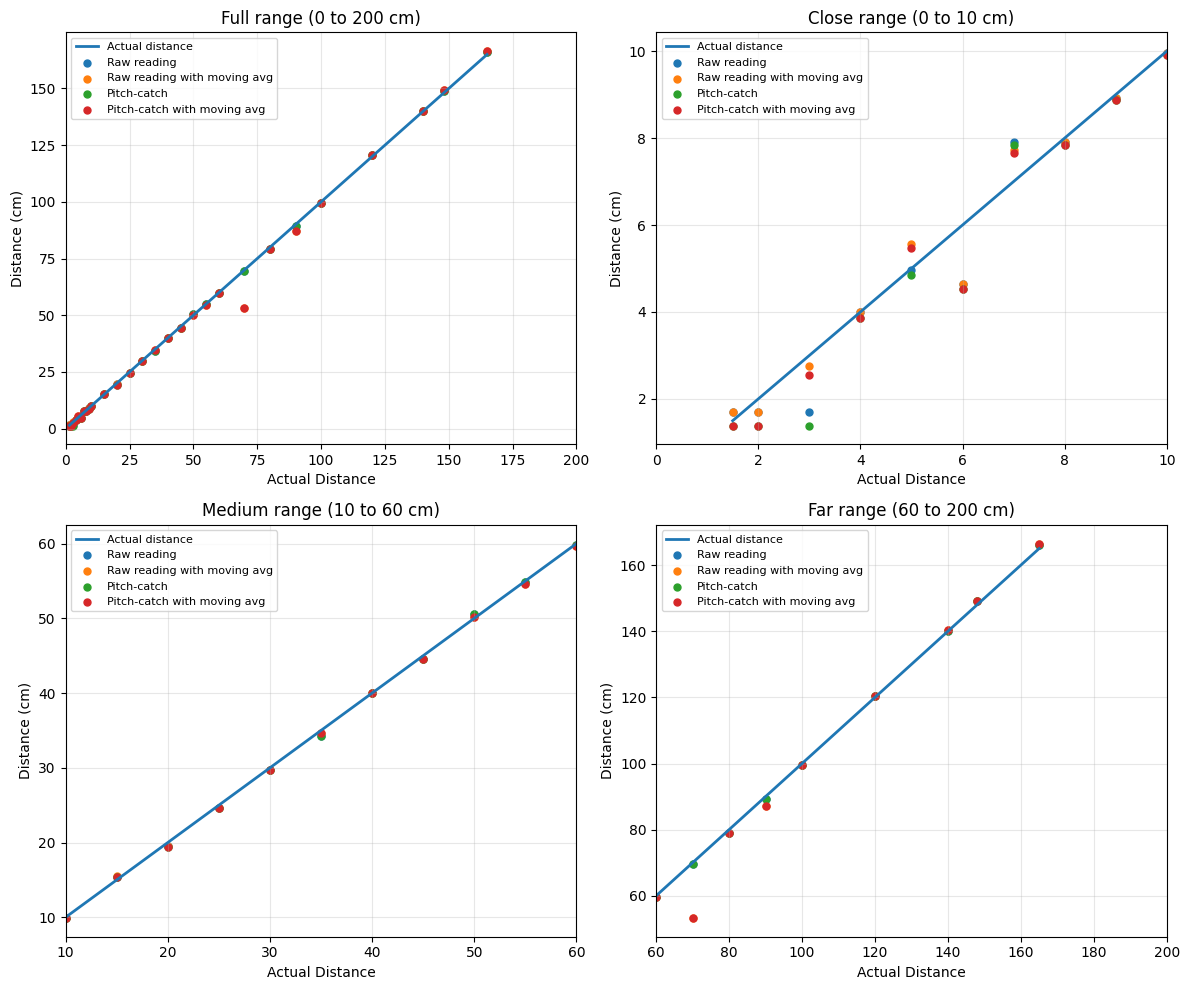
\includegraphics[width=0.95\linewidth]{figures/sensor reading plots across different distances.png}
\caption{Sensor reading plots across different distances.}
\label{fig:sensor_reading_plots}
\end{figure}

\begin{figure}[!t]
\centering
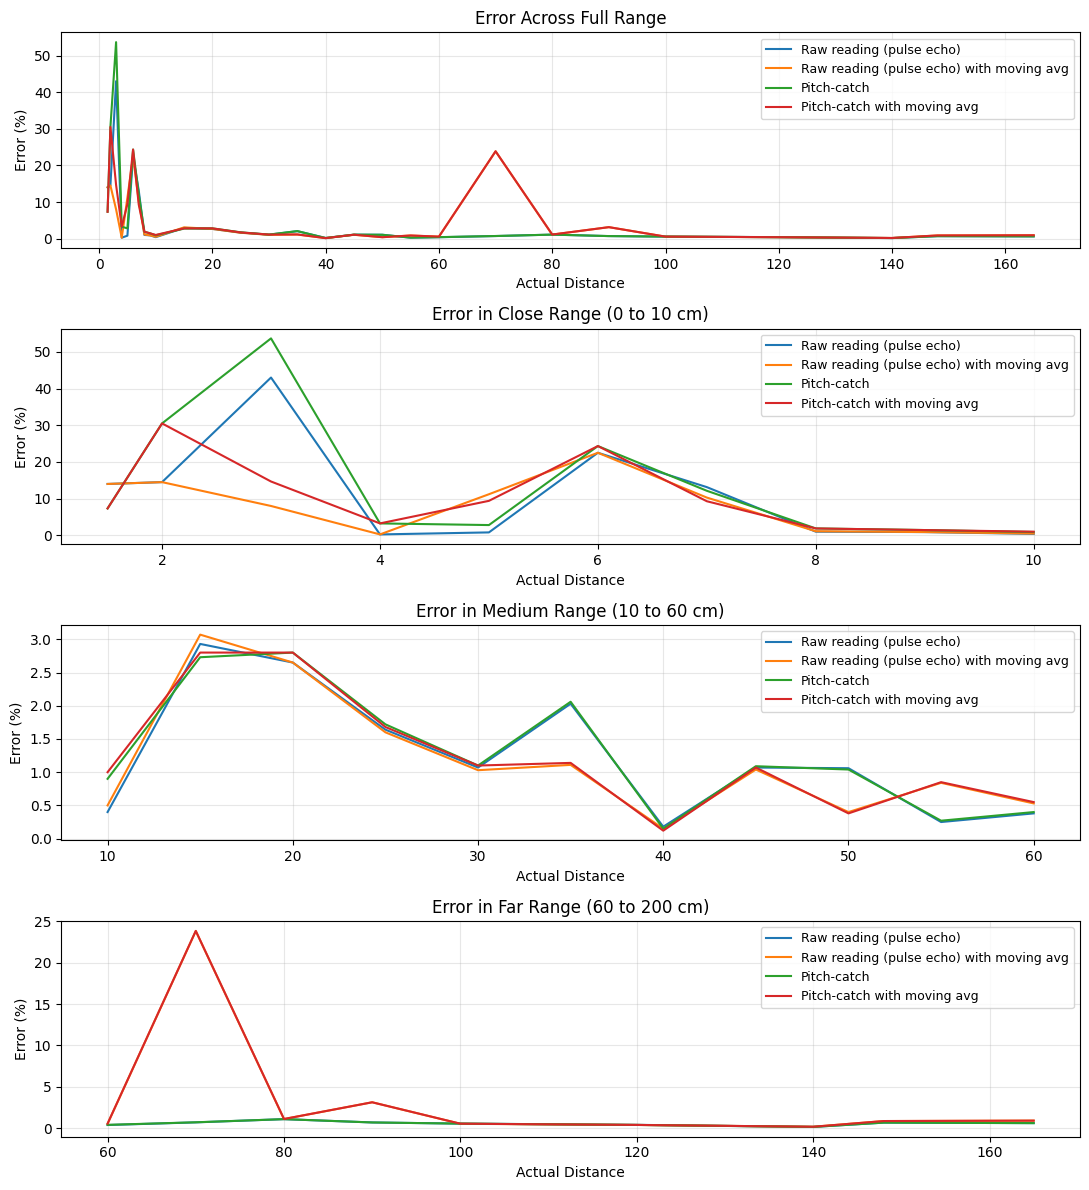
\includegraphics[width=0.95\linewidth]{figures/error plots across different distances.png}
\caption{Error plots across different distances for the measured data.}
\label{fig:error_plots}
\end{figure}

\begin{figure}[!t]
\centering
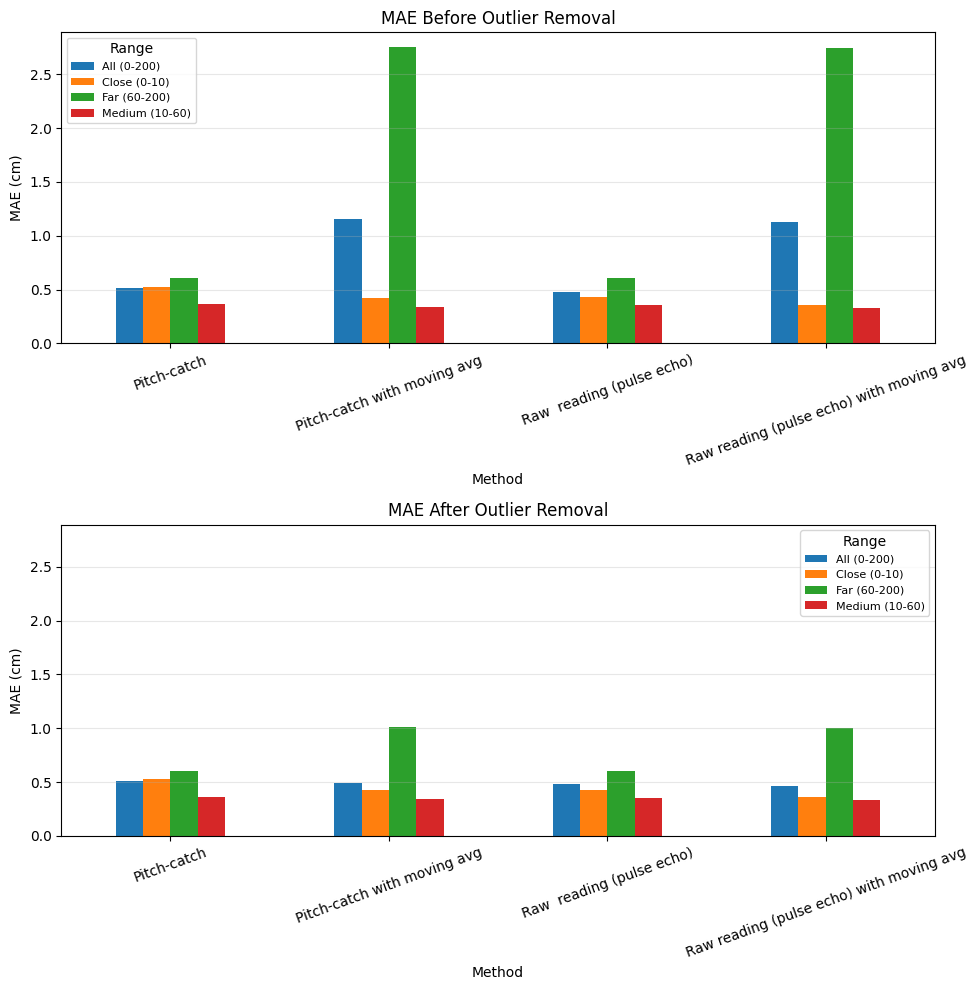
\includegraphics[width=0.95\linewidth]{figures/mean absolute error at different ranges for choosing the best method.png}
\caption{Mean absolute error at different distance ranges for selecting the best measurement method.}
\label{fig:mae_ranges}
\end{figure}

\begin{figure}[!t]
\centering
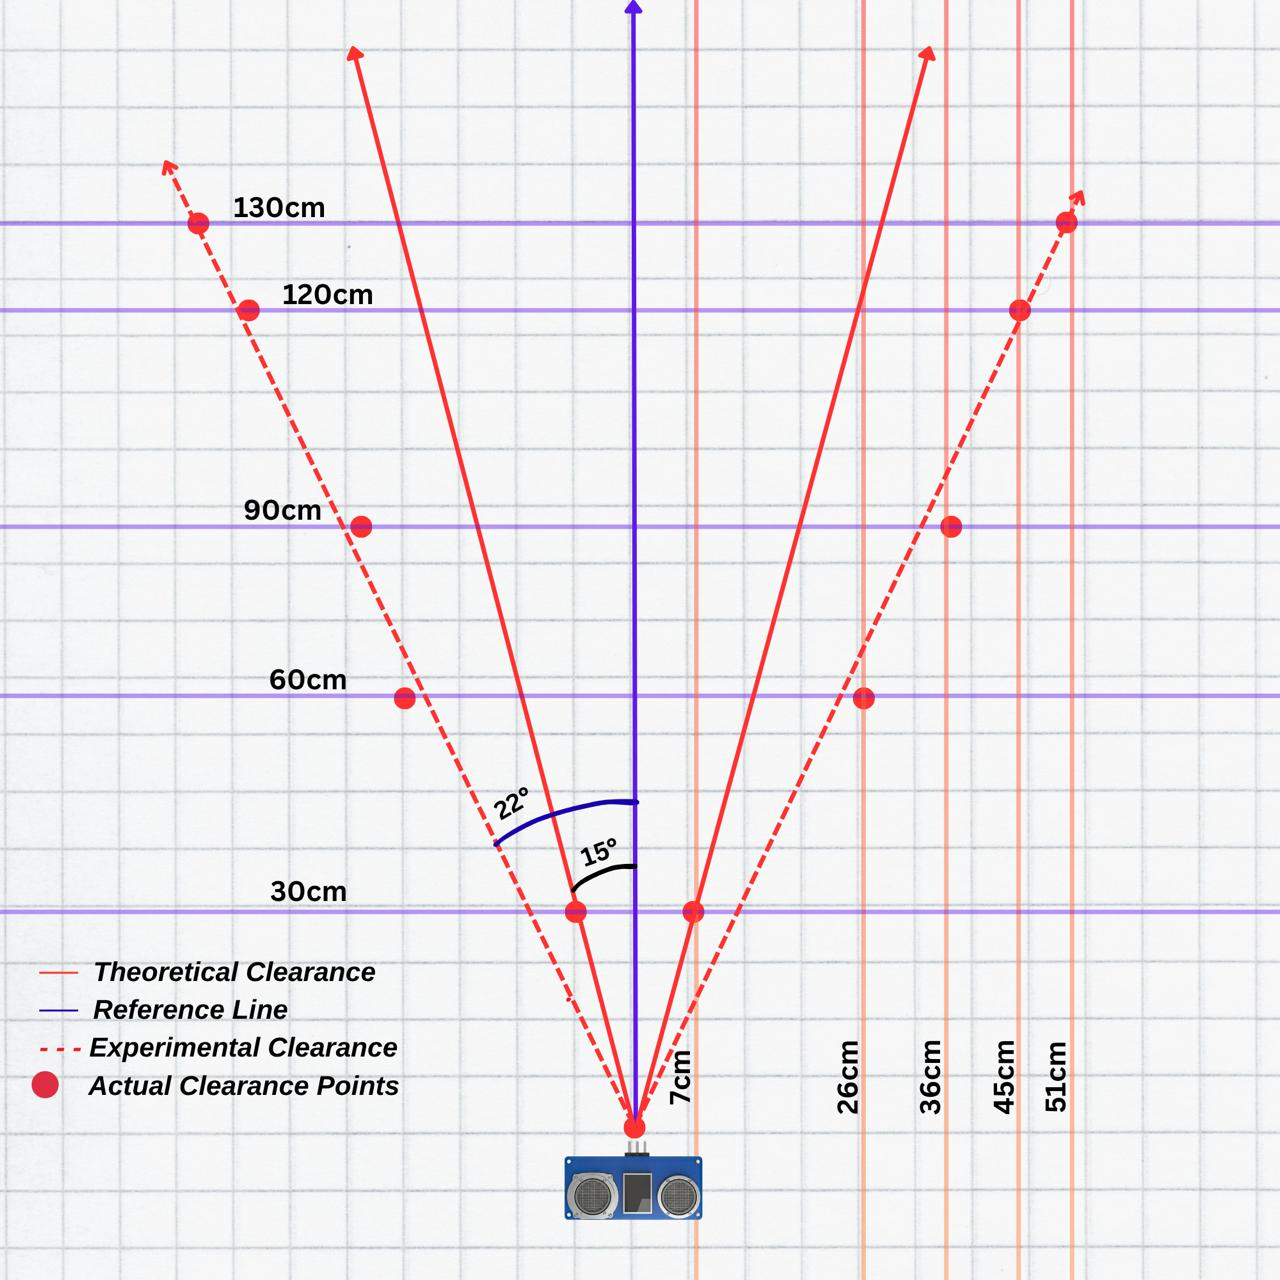
\includegraphics[width=0.95\linewidth]{figures/measuring angle and clearance calculation.jpeg}
\caption{Measurement angle and clearance plot}
\label{fig:clearance_calculation}
\end{figure}

\section{Error Analysis and Discussion}
The main sources of error in this work are likely related to
measurement setup and sensor behavior. Larger
deviations appear mainly at short distances and at a few isolated
outlier points, suggesting that the error is not caused by one factor
alone.

One possible source is human error during measurement and calibration.
Small inaccuracies in setting the reference distance, reading the scale,
or entering the calibration value into the firmware may affect the
calculated correction factor. Parallel alignment error between the
sensor and the target surface may also influence the time-of-flight by
changing the effective reflection path.

Environmental conditions may also contribute to the observed
differences. Since the speed of sound depends on temperature and
humidity, variations in the surrounding air can affect the measured
distance. In this work, these effects were handled mainly through
calibration, and they could be reduced further by incorporating
additional environmental sensors in future implementations. Unwanted
reflections, acoustic disturbance, and nearby obstacles may also
introduce noise into the received signal.

Sensor and circuit limitations may be another reason for the remaining
error. Timing jitter, inconsistent echo detection, or reduced response
stability at some distances may produce abnormal samples. This may
explain why some moving-average results become worse when outliers are
present.

The clearance results also suggest a practical geometric limitation.
Although the system was able to detect distance up to 165~cm, the
required clearance increases with distance because of beam spreading. A
theoretical measurement angle of about $15^\circ$ appears to be
reasonable only within the first 30~cm, while the experimental pattern
after that region is closer to about $22^\circ$. If a maximum allowable
clearance of 30~cm is imposed in the path of flight, the practical
usable range would be limited to approximately 90~cm even though the
sensor can still detect targets beyond that distance.

Thus, the observed errors may be associated with a combination of human
measurement uncertainty, parallel alignment error, environmental
variation, and sensor noise. Other factors may also be present in the
experimental setup. For this reason, the present system may be less
appropriate for precision-critical applications, while remaining
practically useful in tasks where an uncertainty of roughly
$\pm 0.45$~cm is acceptable.

\section{Conclusion}
An ESP32-based ultrasonic digital range finder was designed,
implemented, and calibrated successfully. The results show that both
pulse-echo and pitch-catch processing can provide useful distance
measurements, with better consistency in the medium and far ranges than
at very short distances. Although accurate measurements were achieved up to
165~cm, the clearance study suggests that, under a practical maximum
clearance constraint of 30~cm, the effective usable range is about
90~cm. The observed average tolerance indicates that the system is more
suitable for applications with about $\pm 0.45$~cm allowable error than
for precision-critical measurement tasks. Nevertheless, the prototype
shows good potential for applications such as object detection and
object trajectory estimation. Future improvement may be achieved
through better sensor alignment, more stable mounting, and stronger
filtering or outlier-handling methods.

\begin{thebibliography}{1}
\providecommand{\url}[1]{#1}
\csname url@samestyle\endcsname
\providecommand{\newblock}{\relax}
\providecommand{\bibinfo}[2]{#2}
\providecommand{\BIBentrySTDinterwordspacing}{\spaceskip=0pt\relax}
\providecommand{\BIBentryALTinterwordstretchfactor}{4}
\providecommand{\BIBentryALTinterwordspacing}{\spaceskip=\fontdimen2\font plus
\BIBentryALTinterwordstretchfactor\fontdimen3\font minus \fontdimen4\font\relax}
\providecommand{\BIBforeignlanguage}[2]{{%
\expandafter\ifx\csname l@#1\endcsname\relax
\typeout{** WARNING: IEEEtran.bst: No hyphenation pattern has been}%
\typeout{** loaded for the language `#1'. Using the pattern for}%
\typeout{** the default language instead.}%
\else
\language=\csname l@#1\endcsname
\fi
#2}}
\providecommand{\BIBdecl}{\relax}
\BIBdecl

\bibitem{mi13040520}
\BIBentryALTinterwordspacing
Z.~Qiu, Y.~Lu, and Z.~Qiu, ``Review of ultrasonic ranging methods and their current challenges,'' \emph{Micromachines}, vol.~13, no.~4, 2022. [Online]. Available: \url{https://www.mdpi.com/2072-666X/13/4/520}
\BIBentrySTDinterwordspacing

\bibitem{esp32_datasheet}
\BIBentryALTinterwordspacing
{Espressif Systems}, \emph{ESP32 Series Datasheet}, 2023. [Online]. Available: \url{https://www.espressif.com/sites/default/files/documentation/esp32_datasheet_en.pdf}
\BIBentrySTDinterwordspacing

\bibitem{wokwi_simulation}
{Wokwi}, \url{https://wokwi.com/projects/460254579987104769}, 2026, online simulation file used during circuit verification.

\bibitem{eee354_github_repo}
S.~R. Hassan and A.~Rahman, ``Eee-354-project,'' \url{https://github.com/SrhTurjo/EEE-354-Project}, 2026, gitHub repository for the project software and ESP32 firmware.

\bibitem{HC-SR04_datasheet}
\BIBentryALTinterwordspacing
E.~Freaks, \emph{HC-SR04 Ultrasonic Sensor Datasheet}, 2020. [Online]. Available: \url{https://cdn.sparkfun.com/datasheets/Sensors/Proximity/HCSR04.pdf}
\BIBentrySTDinterwordspacing

\end{thebibliography}

\end{document}
